\chapter{Transient conduction problems}
\section{Overview}
This chapter mainly discussed how to solve transient problems, including lumped method, the general method for different shape’s transient problem, and also how to use the FEM methods to solve fin transient problems.
\section{The lumped capacitance method}

\begin{example}
\textbf{Lumped method and steady state}
\textcolor{blue} {\emph{Refer to tutorial Square - Exact Solution.nb, and Ch. 5, P. 281.}}
Consider a plane wall with consist internal temperature $T_i$ was quickly put into an 
environment surrounded with symmetrically fluids with constant temperature $T_\infty$. 
Wall thickness is $2L_c$. The density of the wall is $\rho=921kg/m^3 $,
the specific heat capacity is $c=2100J/kg\cdot K, k=2.0W/m\cdot K$. The covection coefficient between the junction surface and the
gas is $h=200W/m^2\cdot K$. 3 groups of parameters are given below and 
calculate the temperature difference changed with time compared to the initial temperature difference, use lumped method and steady state method, and compare the results difference. (As shown in figure \ref{fig:4:1})
$$\frac{\theta}{\theta_i}=\frac{T-T_\infty}{T_i-T_\infty}$$
\begin{enumerate}
\item Case 1: $L_{c1}=0.001 m, Bi_A=0.1, C_{1A}=1.016$ and \\
$\zeta_{1A}=0.311 rad, \text{ time } t=60s$
\item Case 2: $L_{c2}=0.01 m, Bi_B=0.1, C_{1B}=1.1191$ and \\
$\zeta_{1B}=0.8603 rad, \text{ time } t=600s$
\item Case 3: $L_{c3}=0.1 m, Bi_C=10.0, C_{1C}=1.2620$ and \\
$\zeta_{1C}=1.4289 rad, \text{ time } t=22000s$
\end{enumerate}
\end{example}
\begin{solution}
~\\
Based on lumped capacitance method, internal temperature of the wall is constant; the plane wall with convection’s temperature distribution is expressed as
$$\frac{\theta}{\theta_i}=
\frac{T-T_\infty}{T_i-T_\infty}=exp(-Bi\cdot Fo)
$$
Where
$$Fo=\frac{\alpha t}{{L_c}^2}$$
$$\alpha=\frac{k}{\rho c}$$
And for general solution of plane wall convection transient problem, the shape effect is required to be considered, the temperature at the centerline of the plane wall
$${\theta_0}^*=\frac{\theta_0}{\theta_i}
=\frac{T-T_\infty}{T_i-T_\infty}=C_1 exp(-\zeta^2Fo)
$$
So that we can plot the internal temperature of the plane wall for the 3 conditions listed above. From figure \ref{fig:4:2}, figure \ref{fig:4:3} and figure \ref{fig:4:4}, we can see that the lumped capacitance method is closed to general solution only when $B_i<0.1$

\begin{figure}[H]
  \centering
    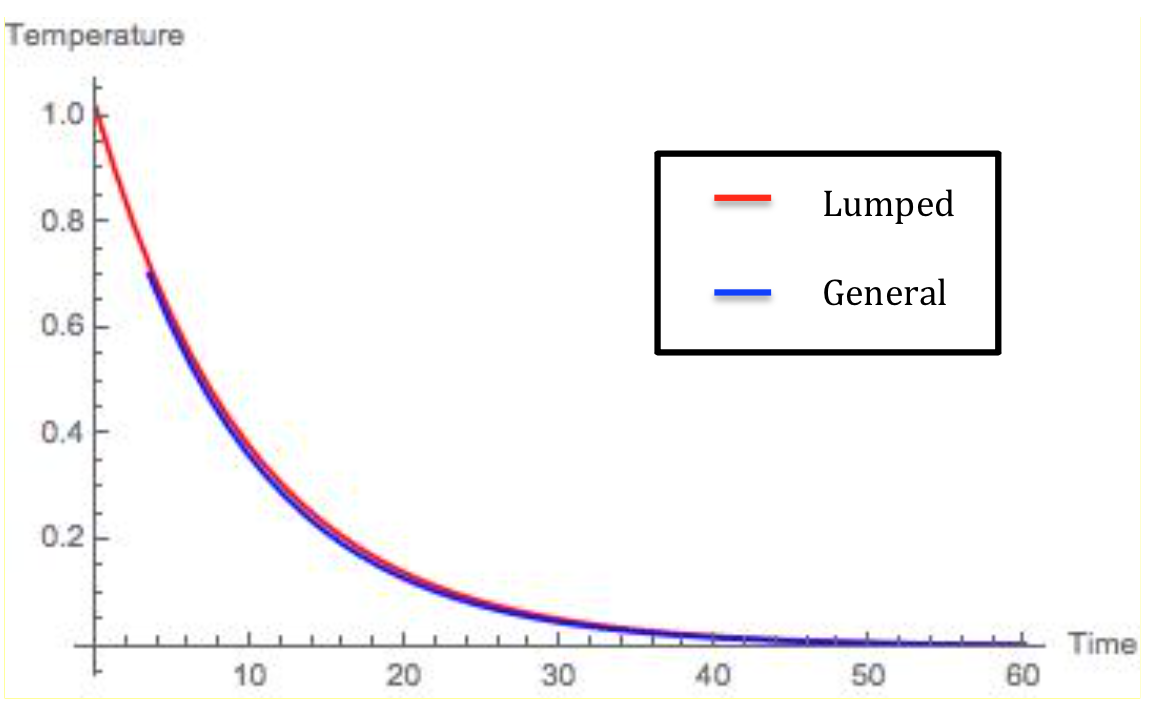
\includegraphics[scale=0.8]{figures/ch4/2}
    \caption{case 1 when $L_{c1}=0.001 m$}
    \label{fig:4:2}
\end{figure}

\begin{figure}[H]
  \centering
    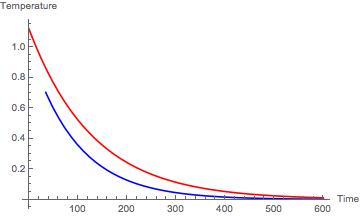
\includegraphics[scale=0.8]{figures/ch4/3}
    \caption{case 2 when $L_{c2}=0.01 m$}
    \label{fig:4:3}
\end{figure}

\begin{figure}[H]
  \centering
    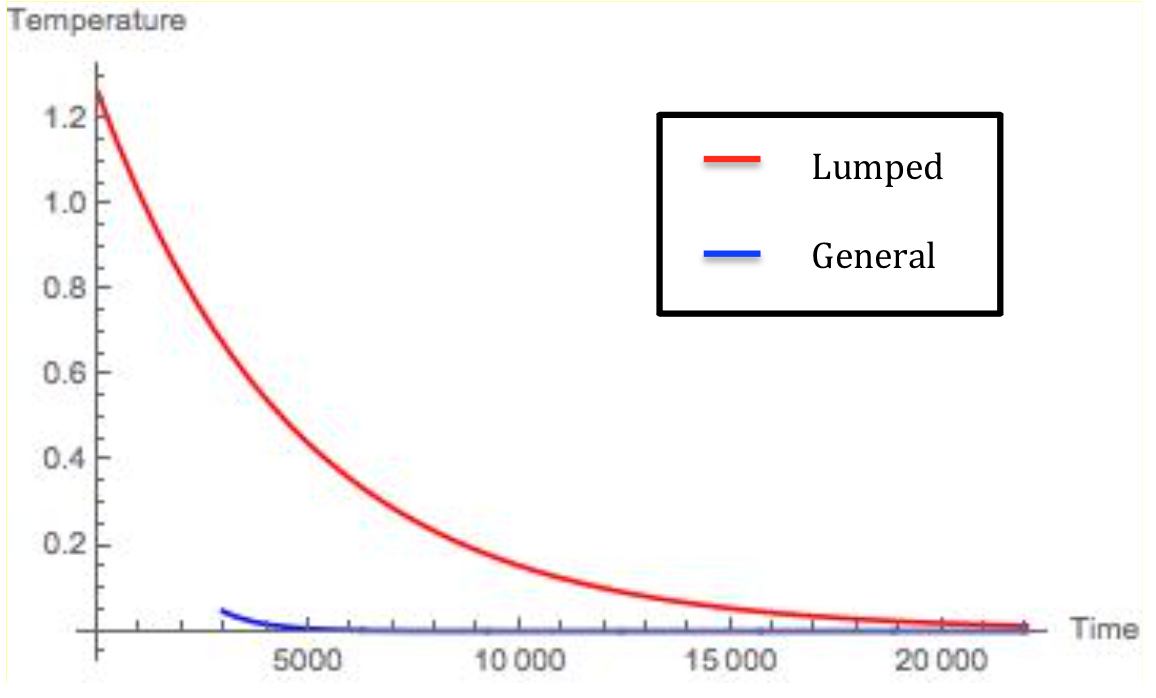
\includegraphics[scale=0.8]{figures/ch4/4}
    \caption{case 3 when $L_{c3}=0.1 m$}
    \label{fig:4:4}
\end{figure}
\end{solution}

\section{FEM method for fin problem}
\begin{example}
\label{example:4:FEM}
Consider a fin length is $L = 0.04 m$, width $w = 0.01$, thickness $THICK = 1 m. h = 10 W/m^2 C, k = 3 W/mC, Cp = 450 J/kg C$,
density $DENS = 8000 kg/m^3$. At $t=0$, the fin temperature at $x=0 $is $T_0=30\circ C$,
the fin is suddenly put into a environment with Tenv=20 0C, at x=L, the temperature keeps as $40\circ C$.
Use RC method to get the transient temperature in the fin. (Shown in figure \ref{fig:4:5})
\begin{figure}[H]
  \centering
    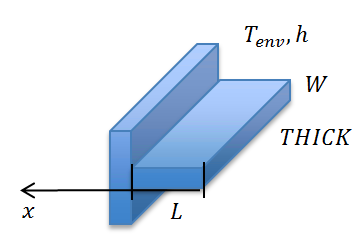
\includegraphics[scale=0.8]{figures/ch4/5}
    \caption{model of example \ref{example:4:FEM}}
    \label{fig:4:5}
\end{figure}
\end{example}

\begin{solution}
~\\
Chose $\Delta X=0.01 m$, $\Delta T=2.5 s$. Build the energy balance equation for each node
As shown in figure \ref{fig:4:6}.
\begin{figure}[H]
  \centering
    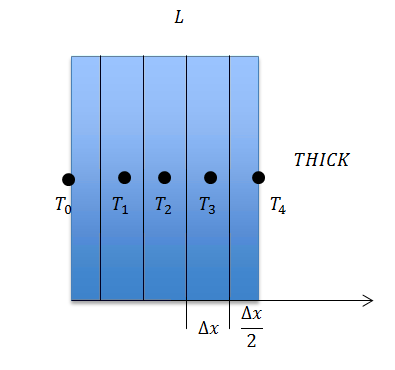
\includegraphics[scale=0.8]{figures/ch4/6}
    \caption{unit node with convection and one-dimensional transient conduction}
    \label{fig:4:6}
\end{figure}
Build the energy balance equation for each node from time $px\Delta T$ to $(p+1)\Delta T$
$$
hA_s(T_{env}-{T_1}^p)+\frac{kA_c}{\Delta x}(T_0-{T_1}^p)+
\frac{kA_c}{\Delta x}({T_2}^p-{T_1}^p)=
\rho c \Delta V\frac{{T_1}^{p+1}-{T_1}^p}{\Delta t}
$$
$$
hA_s(T_{env}-{T_2}^p)+\frac{kA_c}{\Delta x}({T_1}^p-{T_2}^p)+
\frac{kA_c}{\Delta x}({T_3}^p-{T_2}^p)=
\rho c \Delta V\frac{{T_2}^{p+1}-{T_2}^p}{\Delta t}
$$
$$
hA_s(T_{env}-{T_3}^p)+\frac{kA_c}{\Delta x}({T_2}^p-{T_3}^p)+
\frac{kA_c}{\Delta x}({T_4}^p-{T_3}^p)=
\rho c \Delta V\frac{{T_3}^{p+1}-{T_3}^p}{\Delta t}
$$
$${T_4}^{p+1}={T_4}^p=40$$

Where $A_s=p\cdot \Delta x=2\cdot (THICK+w)\cdot\Delta x$ is the surface area for unit 1, 2, 3.
$A_c=THICK\cdot w$ is the cross sectional area for each unit. $\Delta V=A_c\cdot \Delta x$ is the unit volume for unit 1, 2, 3.

\textbf{RC Method:} 
Resistance to convection  transfer is $R_{env}=1/hA_s$ resistance to heat conduction is
$R_i=\Delta x/kA_c$. Lumped thermal capacitance $C_i=\rho c\Delta V$.
So the energy balance equation could be written as
$$
{T_1}^{p+1}=\frac{\Delta t}{C_i}
\left(
\frac{{T_0}-{T_1}^p}{R_i}+
\frac{{T_2}^p-{T_1}^p}{R_i}+
\frac{T_{env}-{T_1}^p}{R_{env}}
\right)
$$
$$
{T_2}^{p+1}=\frac{\Delta t}{C_i}
\left(
\frac{{T_1}-{T_2}^p}{R_i}+
\frac{{T_3}^p-{T_2}^p}{R_i}+
\frac{T_{env}-{T_2}^p}{R_{env}}
\right)
$$
$$
{T_1}^{p+1}=\frac{\Delta t}{C_i}
\left(
\frac{{T_2}-{T_3}^p}{R_i}+
\frac{{T_4}^p-{T_3}^p}{R_i}+
\frac{T_{env}-{T_3}^p}{R_{env}}
\right)
$$
$${T_4}^{p+1}={T_4}^p=40$$
\textbf{Normal method:}
Use the Biot number and finite-difference form of the Fourier number.
$$Fo=\frac{\alpha\Delta t}{(\Delta x)^2}$$
$${Fo}_2=\frac{\alpha\Delta t}{A_c}$$
$$Bi=h\cdot p/k $$
Where thermal diffusivity $\alpha=k/\rho C_p$. The normal form energy balance
equation for the 4 nodes are
$$
{T_1}_{p+1}=(1-2Fo-Bi{Fo}_2)\cdot {T_1}^p+
Fo(T_0+{T_2}^p)+B_i\cdot {Fo}_2\cdot T_{env}
$$
$$
{T_2}_{p+1}=(1-2Fo-Bi{Fo}_2)\cdot {T_2}^p+
Fo({T_1}^p+{T_3}^p)+B_i\cdot {Fo}_2\cdot T_{env}
$$
$$
{T_3}_{p+1}=(1-2Fo-Bi{Fo}_2)\cdot {T_3}^p+
Fo({T_2}^p+{T_4}^p)+B_i\cdot {Fo}_2\cdot T_{env}
$$
$${T_4}^{p+1}={T_4}^p$$

$T_0= 
\begin{bmatrix}
{T_1}^0\\
{T_2}^0\\
{T_3}^0\\
{T_4}^0\\
\end{bmatrix}
=
\begin{bmatrix}
30\\
30\\
30\\
30\\
\end{bmatrix}
$

$T_{100}=
\begin{bmatrix}
31.029\\
32.9242\\
35.8654\\
40\\
\end{bmatrix}
$
\end{solution}


